% Central Overleaf rewrite of
%   William Chang, ``Wasserstein Gradient Flows for Mean-Field Market Making''
%
% Upload THIS file as the main Overleaf document. Put the eight figures in a
% figs/ folder next to it (or keep the repo layout: this file in paper/,
% figures in ../figs/).
%
% What changed relative to Wasserstein_finance.pdf:
%   * experiments are numerical verification, not market evidence;
%   * b is a cross-sectional dispersion penalty, not ``crowding = similar inventories'';
%   * JKO keeps mass/positivity/energy dissipation without CFL; no equal-resolution
%     accuracy claim;
%   * empirical program = moment restrictions + W2 forecasts + local alignment.
% Theory (Props.~6--8, Thms.~7 and~9, Appendix) is unchanged except the reading of b.

\documentclass[11pt]{article}

\usepackage[margin=1in]{geometry}
\usepackage{amsmath,amssymb,amsthm,mathtools}
\usepackage{graphicx}
\usepackage[numbers]{natbib}
\usepackage{booktabs}
\usepackage{microtype}
\usepackage[colorlinks,citecolor=blue,linkcolor=blue,urlcolor=blue]{hyperref}
\usepackage{xcolor}

\graphicspath{{../figs/}{figs/}{./}}

\newtheorem{theorem}{Theorem}
\newtheorem{proposition}[theorem]{Proposition}
\newtheorem{definition}[theorem]{Definition}
\newtheorem{remark}[theorem]{Remark}

\newcommand{\R}{\mathbb{R}}
\newcommand{\Ptwo}{\mathcal{P}_2}
\newcommand{\Wtwo}{W_2}
\newcommand{\dx}{\,dx}
\newcommand{\dt}{\,dt}

\title{Wasserstein Gradient Flows for Mean-Field Market Making}
\author{William Chang\\
Department of Applied Mathematics\\
University of California, Los Angeles\\
\texttt{https://williamc.me/}}
\date{}

\begin{document}
\maketitle

\begin{abstract}
Financial markets do not literally minimize a physical energy, but the distribution
of strategic agents in a market may evolve toward equilibria that minimize a
cost-like free-energy functional. This project studies a mean-field market-making
model in which the population distribution of dealer inventories evolves under the
combined effect of an inventory/risk penalty, a pairwise interaction, and an
entropic dispersion term. For the quadratic kernel
$W(x,y)=\frac{b}{2}(x-y)^2$ with $b>0$, the interaction
\emph{penalizes cross-sectional dispersion} and synchronizes inventories; it is
not a penalty on dealers holding similar positions. We formulate the
Fokker--Planck side of the population dynamics as a Wasserstein gradient flow
whenever the interaction structure is potential, and we discretize the evolution
with a Jordan--Kinderlehrer--Otto (JKO) proximal scheme. Numerical experiments
verify the analytic predictions of the quadratic model and the structural
guarantees of JKO. They are not empirical evidence that dealer inventories in
real markets follow these dynamics. A separate suite of synthetic
diagnostics---moment restrictions, distributional forecasts, and local directional
alignment---is developed as a template for a future test on observable
market-state distributions.
\end{abstract}

\section{Introduction}

A recurring intuition imported from physics into quantitative finance is that
``systems evolve toward states of lower energy.'' Taken literally at the level of
prices or returns, the analogy fails: raw asset returns are heavy-tailed,
nonstationary, and carry no natural notion of a scalar energy that they decrease
over time. The object that \emph{does} admit such a description is not the price
but the \emph{distribution of agent states}---dealer inventories, beliefs, risk
exposures, or order-flow intensities---which can plausibly relax toward an
equilibrium that minimizes a cost-like functional. The natural geometry for this
relaxation is not Euclidean but the Wasserstein geometry of optimal transport, in
which a distribution evolves by transporting probability mass at minimal kinetic
cost.

This shift of viewpoint is what makes the physical analogy precise. The seminal
observation of~\cite{JKO98} is that the Fokker--Planck equation can be written as
the gradient flow, \emph{in the $2$-Wasserstein metric}, of a free-energy
functional: a density $\rho_t$ moves in the direction of steepest descent of an
energy $F$, subject to the cost of transporting mass. Their variational
time-discretization---now called the JKO scheme---replaces the PDE by a sequence
of minimizations of ``energy plus transport cost,''
\begin{equation}
\label{eq:jko}
\rho_{k+1}
\in
\arg\min_{\rho\in\Ptwo(\R^d)}
\left\{
F(\rho)+\frac{1}{2\tau}\Wtwo^2(\rho,\rho_k)
\right\},
\end{equation}
which is exactly the statement ``the next state is a low-energy state, penalized
for moving too far too fast.'' This is the structure we wish to exploit on the
finance side.

\paragraph{Why market making.}
Mean-field games (MFGs) provide a setting in which a distribution of strategic
agents genuinely evolves toward equilibrium. In the market-making model
of~\cite{GueantLehalleFernandez2013}, a market maker quotes against a continuum
of strategic market takers whose aggregate behavior enters through a mean-field
interaction; the equilibrium is characterized by a coupled
Hamilton--Jacobi--Bellman (HJB) and Fokker--Planck system. The Fokker--Planck
half of that system governs precisely the population density that our free-energy
picture is meant to describe. Inventory is the natural state variable: market
makers dislike large positions, pairwise interaction can synchronize inventories
across dealers, and exogenous order flow tilts the landscape that the inventory
distribution relaxes within. Each of these effects has a clean counterpart in a
free-energy functional, which is what makes the analogy concrete rather than
decorative.

\paragraph{The central caveat.}
It is tempting to assert that ``the Fokker--Planck half of an MFG \emph{is} a
Wasserstein gradient flow.'' This is too strong. In a general MFG the forward
equation is a continuity equation driven by the optimal feedback control coming
from the HJB equation,
\begin{equation}
\label{eq:mfg-fp}
\partial_t m
-\nabla\cdot\bigl(m\,D_p H(x,\nabla u,m)\bigr)
-\nu\Delta m
=0,
\end{equation}
and such a drift need not be the gradient of the first variation of any scalar
energy. The Fokker--Planck equation becomes a bona fide Wasserstein gradient flow
only under additional structure---for instance potential (variational) MFG
structure, entropic regularization, or convex costs whose induced drift can be
written as $-\nabla\delta F/\delta m$. We therefore do not claim that mean-field
market making is ``automatically JKO.'' We instead pose the design question:

\begin{remark}[Scope of the analogy]
\label{rem:scope}
We seek to \emph{identify or design} a market-making mean-field game whose
population dynamics admit a Wasserstein-gradient-flow (equivalently, a
generalized JKO) formulation, and to use that structure for stable computation
and for interpretability of the resulting equilibria. The energy lives on the
distribution of \emph{agent states}, never on raw prices or returns.
\end{remark}

\paragraph{Contributions.}
Within this scope, the project proceeds as follows.
\begin{enumerate}
\item We formulate a free-energy functional $F$ on the distribution of dealer
inventories that combines an inventory/risk potential, a pairwise interaction,
and an entropic term, and we record the precise conditions under which the
associated Fokker--Planck dynamics are the $W_2$-gradient flow of $F$
(Section~\ref{sec:prelim}).
\item We discretize the flow with the JKO scheme~\eqref{eq:jko} and compare it
to standard Fokker--Planck integrators, checking energy dissipation, conservation
of mass and positivity, and large-step stability. We do not claim accuracy gains
at equal spatial resolution.
\item We study comparative statics of the equilibrium inventory distribution in
the interaction strength $b$ and the entropy weight $\beta$, and the transient
response to exogenous liquidity shocks modelled as time-dependent tilts of the
potential. A separate suite of synthetic diagnostics (moment restrictions,
distributional forecasts, and local directional alignment) is developed as a
template for a future test on observable market-state distributions; it is not
itself that test.
\end{enumerate}

\paragraph{Related work.}
The variational formulation of the Fokker--Planck equation is due
to~\cite{JKO98}; the metric-geometric theory of gradient flows in the space of
probability measures is developed in~\cite{AGS08}, with the formal Riemannian
(``Otto'') calculus introduced in~\cite{Otto01} and surveyed
in~\cite{Villani03,Santambrogio15}. The mean-field game framework originates
with~\cite{LasryLions07}; see~\cite{CardaliaguetNotes} for the coupled
HJB--Fokker--Planck system and the notion of potential games. Our market-making
model follows the strategic mean-field formulation of~\cite{GueantLehalleFernandez2013},
itself built on the inventory-control approach of~\cite{AvellanedaStoikov08}. On
the algorithmic side,~\cite{JKOflow} analyze JKO-type proximal descent in
Wasserstein space, which informs our choice of numerical scheme. Finally,
Wasserstein distances have been used directly for regime and change-point
detection in high-dimensional series~\cite{HorvathKokoszka}; we return to this as
an honest, structure-light alternative to monitoring a JKO residual.

\paragraph{Outline.}
Section~\ref{sec:prelim} collects the required preliminaries. Section~\ref{sec:results}
states the one-dimensional quadratic results. Section~\ref{sec:experiments}
numerically verifies the model and the JKO discretization.
Section~\ref{sec:diagnostics} records a synthetic template for a future empirical
test. Proofs are in Appendix~\ref{app:proofs}.

\section{Preliminaries}
\label{sec:prelim}

Throughout, $\Ptwo(\R^d)$ denotes the set of Borel probability measures on
$\R^d$ with finite second moment. Densities are written $\rho$, $m$ and
identified with the corresponding measures when absolutely continuous with
respect to Lebesgue measure. We write $f\ast\rho$ for convolution and $D_p H$
for the gradient of a Hamiltonian $H$ in its momentum slot.

\subsection{Optimal transport and the Wasserstein space}

\begin{definition}[$2$-Wasserstein distance]
For $\mu,\nu\in\Ptwo(\R^d)$, the squared $2$-Wasserstein distance is
\begin{equation}
\label{eq:w2}
\Wtwo^2(\mu,\nu)
=
\inf_{\gamma\in\Pi(\mu,\nu)}
\int_{\R^d\times\R^d}
|x-y|^2\,d\gamma(x,y),
\end{equation}
where $\Pi(\mu,\nu)$ is the set of couplings of $\mu$ and $\nu$.
\end{definition}

The metric space $(\Ptwo(\R^d),\Wtwo)$ is the central object of the
theory~\cite{Villani03,AGS08}. Its dynamic characterization is due
to~\cite{BenamouBrenier00}:
\begin{equation}
\label{eq:bb}
\Wtwo^2(\mu,\nu)
=
\inf_{(\rho_t,v_t)}
\int_0^1\int_{\R^d}|v_t(x)|^2\rho_t(x)\,dx\,dt,
\quad
\partial_t\rho_t+\nabla\cdot(\rho_t v_t)=0,
\quad
\rho_0=\mu,\;\rho_1=\nu,
\end{equation}
the infimum being over curves in $\Ptwo$ joined by a velocity field through the
continuity equation. Equation~\eqref{eq:bb} endows $\Ptwo$ with a formal
Riemannian structure~\cite{Otto01}: tangent vectors at $\rho$ are represented by
velocity potentials $\phi$ via $\partial_t\rho=-\nabla\cdot(\rho\nabla\phi)$,
with metric
$\langle\partial_t^{(1)}\rho,\partial_t^{(2)}\rho\rangle_\rho
=\int\nabla\phi_1\cdot\nabla\phi_2\,\rho\,dx$.
This is the geometry in which the gradient flows below are defined.

\subsection{Free-energy functionals and Wasserstein gradient flows}

We consider free-energy functionals of~\cite{JKO98} type, comprising a
potential, an interaction, and an internal (entropic) term:
\begin{equation}
\label{eq:F}
F(\rho)
=
\int_{\R^d} V(x)\rho(x)\,dx
+
\frac12
\iint_{\R^d\times\R^d}
W(x,y)\rho(x)\rho(y)\,dx\,dy
+
\beta\int_{\R^d}\rho(x)\log\rho(x)\,dx,
\end{equation}
with $V$ a confining potential, $W$ a symmetric interaction kernel, and
$\beta>0$. The first variation of $F$ at $\rho$ is
\begin{equation}
\label{eq:dF}
\frac{\delta F}{\delta\rho}(x)
=
V(x)+(W\ast\rho)(x)+\beta\bigl(\log\rho(x)+1\bigr).
\end{equation}

\begin{definition}[Wasserstein gradient flow]
A curve $(\rho_t)\subset\Ptwo(\R^d)$ is a gradient flow of $F$ in the $W_2$
geometry if it solves
\begin{equation}
\label{eq:gf}
\partial_t\rho_t
=
\nabla\cdot
\left(
\rho_t\nabla\frac{\delta F}{\delta\rho}(\rho_t)
\right).
\end{equation}
\end{definition}

Substituting~\eqref{eq:dF} into~\eqref{eq:gf} yields the nonlinear
Fokker--Planck (McKean--Vlasov) equation
\begin{equation}
\label{eq:mv-general}
\partial_t\rho_t
=
\nabla\cdot\bigl(\rho_t\nabla V\bigr)
+
\nabla\cdot\bigl(\rho_t\nabla(W\ast\rho_t)\bigr)
+
\beta\Delta\rho_t.
\end{equation}
The distribution drifts downhill in the potential $V$ and is dispersed by the
entropic Laplacian. The interaction $W$ is \emph{not} intrinsically repulsive:
its sign and shape decide whether the population spreads or synchronizes. For the
quadratic kernel used below, $W(x,y)=\frac{b}{2}(x-y)^2$ with $b>0$, one has
$\nabla(W\ast\rho)=b(x-\mu)$, so the interaction \emph{pulls inventories toward
the mean}. Along~\eqref{eq:gf} the energy is dissipated at rate
$\frac{d}{dt}F(\rho_t)=-\int\rho_t\bigl|\nabla\delta F/\delta\rho\bigr|^2 dx\le 0$.

\subsection{The JKO minimizing-movement scheme}

The variational time-discretization of~\cite{JKO98} approximates~\eqref{eq:gf}
by the proximal iteration
\begin{equation}
\label{eq:jko-step}
\rho_{k+1}
\in
\arg\min_{\rho\in\Ptwo(\R^d)}
\left\{
F(\rho)+\frac{1}{2\tau}\Wtwo^2(\rho,\rho_k)
\right\},
\qquad
\rho_0=\bar\rho,
\end{equation}
with step size $\tau>0$. As $\tau\to 0$ the piecewise-constant interpolation of
$(\rho_k)$ converges to the gradient flow~\eqref{eq:gf}~\cite{AGS08}; the scheme
is the Wasserstein analogue of the implicit Euler method, and inherits its
unconditional stability, automatic preservation of nonnegativity and total mass,
and monotone energy decrease $F(\rho_{k+1})\le F(\rho_k)$ \emph{on the autonomous
problem}. This is what recommends~\eqref{eq:jko-step} as a numerical method
rather than only a theoretical device.

\subsection{Brenier's theorem and the transport map between JKO iterates}

The iteration~\eqref{eq:jko-step} produces the sequence $(\rho_k)$ as a list of
distributions, but it says nothing directly about \emph{where} mass goes from one
step to the next. Brenier's theorem supplies this missing object.

\begin{theorem}[Brenier~\cite{Brenier91,Villani03}]
\label{thm:brenier}
Let $\mu,\nu\in\Ptwo(\R^d)$ and suppose $\mu$ is absolutely continuous with
respect to Lebesgue measure. Then the infimum in~\eqref{eq:w2} is attained by a
unique coupling, induced by a $\mu$-almost-everywhere unique map
$T:\R^d\to\R^d$: $\nu=T_{\#}\mu$ and
$\Wtwo^2(\mu,\nu)=\int |x-T(x)|^2\,d\mu(x)$. Moreover $T=\nabla\phi$ for a
convex potential $\phi$.
\end{theorem}

Applied with $\mu=\rho_k$ and $\nu=\rho_{k+1}$, there is a unique Brenier map
$T_k$ with $\rho_{k+1}=(T_k)_{\#}\rho_k$. To first order,
\begin{equation}
\label{eq:brenier-disc}
T_k(x)
=
x
-\tau\nabla\frac{\delta F}{\delta\rho}(\rho_{k+1})(x)
+o(\tau),
\end{equation}
so the displacement $T_k-\mathrm{id}$ is proportional to the Wasserstein gradient
evaluated at the new iterate. This identification underlies the alignment
diagnostic of Section~\ref{sec:diagnostics}: given consecutive empirical clouds,
the observed object is the displacement of the two \emph{marginals}, not the
trajectory of labeled dealers unless identities are observed.

\subsection{Mean-field games and the HJB--Fokker--Planck system}

A representative agent with state $X_t\in\R^d$ chooses a control $\alpha_t$ with
dynamics $dX_t=\alpha_t\,dt+\sqrt{2\nu}\,dB_t$ to minimize a cost depending on a
running Lagrangian and on the population $m_t=\mathrm{Law}(X_t)$. At equilibrium
the value function $u$ and the density $m$ solve
\begin{equation}
\label{eq:mfg}
\begin{cases}
-\partial_t u-\nu\Delta u+H(x,\nabla u)=f(x,m),\\
\partial_t m-\nu\Delta m-\nabla\cdot\bigl(m\,D_p H(x,\nabla u)\bigr)=0,\\
m(0,\cdot)=m_0,\quad u(T,\cdot)=g(x,m(T)).
\end{cases}
\end{equation}
As emphasized in Remark~\ref{rem:scope}, the forward equation is a continuity
equation, but its drift $-D_p H(x,\nabla u)$ is determined by the HJB solution
and is not, in general, the Wasserstein gradient of any scalar energy.

\begin{definition}[Potential mean-field game]
\label{def:potential}
The game~\eqref{eq:mfg} is \emph{potential} (variational) if the coupling derives
from a functional, i.e.\ $f(x,m)=\delta G/\delta m$ for some $G$, so
that~\eqref{eq:mfg} arises as the optimality system of a single control-of-PDE
problem. In this case the equilibrium minimizes a global energy, and the forward
dynamics inherit the gradient-flow / JKO structure of the previous subsections.
\end{definition}

This is the precise hypothesis under which the ``systems move toward lower
energy'' picture is rigorous.

\subsection{The mean-field market-making model}
\label{sec:mm}

We instantiate the state $x$ as a dealer's signed inventory and follow the
strategic mean-field market-making setup of~\cite{GueantLehalleFernandez2013}, in
the tradition of inventory-control market making~\cite{AvellanedaStoikov08}. A
market maker quotes bid and ask prices and accumulates inventory from the order
flow generated by a continuum of market takers. For the variational study we
focus on the induced population density $m_t$ of inventories and posit a free
energy~\eqref{eq:F} in which
\begin{itemize}
\item $V$ penalizes large absolute inventory (inventory risk), e.g.\
$V(x)=\frac{a}{2}x^2$, capturing mean reversion of positions toward zero;
\item $W$ is a pairwise interaction. For the quadratic kernel
$W(x,y)=\frac{b}{2}(x-y)^2$ with $b>0$, the interaction
\emph{penalizes cross-sectional dispersion} and synchronizes inventories toward a
common (here, flat) position. It is not a penalty on dealers holding similar
inventories;
\item $\beta$ controls entropic dispersion of inventories across the population;
\item a time-dependent tilt $V_t(x)$ models exogenous liquidity shocks that
transiently push the distribution away from equilibrium.
\end{itemize}
This one-dimensional specification is the toy model on which the JKO scheme is
tested against a direct Fokker--Planck solver. Whether observed market-state
distributions follow $F$ is a separate question, taken up as a template in
Section~\ref{sec:diagnostics}.

\section{Main results}
\label{sec:results}

We now specialize to the one-dimensional inventory model of
Section~\ref{sec:mm}. Throughout we fix the quadratic specification
\begin{equation}
\label{eq:quad}
V(x)=\frac{a}{2}x^2,
\qquad
W(x,y)=\frac{b}{2}(x-y)^2,
\qquad
a>0,\; b\ge 0,\; \beta>0,
\end{equation}
so that, after using
$\frac12\iint W\,\rho\rho=\frac{b}{2}\mathrm{Var}(\rho)$,
\begin{equation}
\label{eq:Fquad}
F(\rho)
=
\frac{a}{2}\int x^2\rho\,dx
+
\frac{b}{2}\mathrm{Var}(\rho)
+
\beta\int\rho\log\rho\,dx.
\end{equation}
All proofs are deferred to Appendix~\ref{app:proofs}.

\subsection{Gradient-flow representation and its scope}

\begin{proposition}[Gradient-flow form of the inventory dynamics]
\label{prop:gf}
The $W_2$ gradient flow~\eqref{eq:gf} of the functional~\eqref{eq:Fquad} is the
nonlinear Fokker--Planck (McKean--Vlasov) equation
\begin{equation}
\label{eq:mv}
\partial_t m_t
=
\partial_x\Bigl(m_t\bigl[(a+b)x-b\mu_t\bigr]\Bigr)
+
\beta\partial_{xx}m_t,
\qquad
\mu_t:=\int x\, m_t(x)\,dx,
\end{equation}
equivalently $\partial_t m_t=-\partial_x(v_t m_t)+\beta\partial_{xx}m_t$ with
velocity $v_t(x)=-(a+b)x+b\mu_t$. If a market-making mean-field game of the
form~\eqref{eq:mfg} is potential in the sense of Definition~\ref{def:potential}, with running and
coupling costs chosen so that the equilibrium feedback induces the drift
$-\nabla(V+W\ast m)$, then the forward Fokker--Planck equation of the game
coincides with~\eqref{eq:mv} and the population of inventories is, exactly, the
Wasserstein gradient flow of $F$.
\end{proposition}

Proposition~\ref{prop:gf} is the precise content of Remark~\ref{rem:scope}: the
variational picture is not a metaphor once the game is potential and the drift is
the gradient of a first variation, and it is \emph{only} then. The quadratic
specification~\eqref{eq:quad} is the simplest instance for which the hypotheses
hold and the resulting flow can be solved in closed form.

\subsection{Structural guarantees of the JKO scheme}

\begin{theorem}[Well-posedness and structure preservation]
\label{thm:jko}
Let $F$ be as in~\eqref{eq:Fquad} and let $\rho_k\in\Ptwo(\R)$ with
$F(\rho_k)<\infty$. For every $\tau>0$:
\begin{enumerate}
\item[(i)] the JKO step~\eqref{eq:jko-step} admits a unique minimizer
$\rho_{k+1}\in\Ptwo(\R)$, which is absolutely continuous with a strictly positive
density;
\item[(ii)] total mass and nonnegativity are preserved exactly;
\item[(iii)] the scheme dissipates energy at every step, with
\begin{equation}
\label{eq:edp}
F(\rho_{k+1})+\frac{1}{2\tau}\Wtwo^2(\rho_{k+1},\rho_k)\le F(\rho_k);
\end{equation}
\item[(iv)] as $\tau\to 0$, the piecewise-constant interpolant of $(\rho_k)$
converges in $C([0,T];\Ptwo(\R))$ to the unique solution of~\eqref{eq:mv} with
initial datum $\rho_0$.
\end{enumerate}
\end{theorem}

Properties (i)--(iii) are structural advantages absent from a naive explicit
discretization of~\eqref{eq:mv}. They hold for the \emph{autonomous} functional.
When $V$ is replaced by a time-dependent tilt $V_t$,~\eqref{eq:edp} need not
hold for the unadjusted $F$; we return to this in
Section~\ref{sec:exp-shock}.

\subsection{Equilibria as McKean--Vlasov--Gibbs fixed points}

\begin{proposition}[Equilibrium characterization]
\label{prop:eq}
A measure $m_\infty\in\Ptwo(\R)$ is a stationary point of the flow~\eqref{eq:gf}
if and only if $\delta F/\delta\rho(m_\infty)$ is constant on
$\mathrm{supp}(m_\infty)$; equivalently $m_\infty$ is a
McKean--Vlasov--Gibbs fixed point,
\begin{equation}
\label{eq:gibbs}
m_\infty(x)
=
\frac1Z\exp\Bigl(-\frac1\beta\bigl(V(x)+(W\ast m_\infty)(x)\bigr)\Bigr).
\end{equation}
\end{proposition}

At equilibrium the inventory distribution is a Boltzmann--Gibbs density in the
effective potential $V+W\ast m_\infty$, where the interaction shifts the
landscape self-consistently.

\subsection{The explicitly solvable Gaussian case}

\begin{theorem}[Gaussian equilibrium and relaxation rates]
\label{thm:gauss}
Under~\eqref{eq:quad} with $a>0$, $b\ge 0$, $\beta>0$:
\begin{enumerate}
\item[(i)] the flow~\eqref{eq:mv} has a unique equilibrium, the centered Gaussian
\begin{equation}
\label{eq:gauss}
m_\infty=N\bigl(0,\sigma_\infty^2\bigr),
\qquad
\sigma_\infty^2=\frac{\beta}{a+b};
\end{equation}
\item[(ii)] the mean $\mu_t$ and variance $\Sigma_t:=\mathrm{Var}(m_t)$ evolve in
closed form,
\begin{equation}
\label{eq:moments}
\mu_t=\mu_0 e^{-at},
\qquad
\Sigma_t
=
\frac{\beta}{a+b}
+
\Bigl(\Sigma_0-\frac{\beta}{a+b}\Bigr)e^{-2(a+b)t},
\end{equation}
so the mean relaxes at rate $a$ and the variance at rate $2(a+b)$;
\item[(iii)] $F$ is $a$-geodesically convex on $(\Ptwo(\R),\Wtwo)$, and
consequently the flow is an $a$-contraction toward equilibrium,
$\Wtwo(m_t,m_\infty)\le e^{-at}\Wtwo(m_0,m_\infty)$, while the JKO iterates
contract as $\Wtwo(\rho_k,m_\infty)\le(1+a\tau)^{-k}\Wtwo(\rho_0,m_\infty)$.
\end{enumerate}
\end{theorem}

Three financial readings follow immediately. First, the equilibrium dispersion
$\sigma_\infty^2=\beta/(a+b)$ \emph{decreases} in the interaction strength $b$: a
larger dispersion penalty compresses the population around flat inventory. We
refer to $b$ as interaction strength or cross-sectional dispersion penalty, not
as anti-crowding. Second, the mean inventory---the aggregate directional position
of the dealer population---is the slowest mode, relaxing only at rate $a$ set by
individual inventory aversion, whereas the dispersion equilibrates faster at rate
$2(a+b)$. Third, a transient liquidity shock modeled as a tilt
$V_t(x)=\frac{a}{2}(x-c_t)^2$ displaces the mean toward $c_t$ and is then erased
at rate $a$.

\section{Experiments}
\label{sec:experiments}

We test the predictions of Section~\ref{sec:results} on the one-dimensional
quadratic model and compare the JKO scheme against direct Fokker--Planck solvers.
Unless stated otherwise we use $a=1$, $b=\tfrac12$, $\beta=\tfrac12$, for which
Theorem~\ref{thm:gauss} gives $\sigma_\infty^2=\beta/(a+b)=1/3$, mean relaxation
rate $a=1$, and variance relaxation rate $2(a+b)=3$.

These experiments are numerical verification of the proposed model and JKO
discretization. They are not empirical evidence that dealer inventories in real
markets follow these dynamics. We keep three claims separate:
\emph{(i)}~the code reproduces the analytic laws;
\emph{(ii)}~JKO inherits the structural guarantees of Theorem~\ref{thm:jko};
\emph{(iii)}~whether observed market-state distributions follow $F$ is left open
(Section~\ref{sec:diagnostics}).

\paragraph{Numerical methods.}
The Eulerian solvers discretize~\eqref{eq:mv} on a uniform grid of the inventory
axis $[-6,6]$ in conservative flux form with upwind advection, central diffusion,
and reflecting (no-flux) boundaries; we use both explicit (forward Euler) and
implicit (backward Euler) time stepping. The JKO solver works in the
one-dimensional Lagrangian coordinate given by the quantile function
$Q=F_\rho^{-1}$, in which $\Wtwo^2(\rho,\rho_k)=\int_0^1(Q-Q_k)^2\,du$ and
\[
  F[Q]
  =
  \frac{a}{2}\int_0^1 Q^2\,du
  +
  \frac{b}{2}\mathrm{Var}[Q]
  -
  \beta\int_0^1 \log Q'(u)\,du.
\]
Each JKO step is a smooth convex program over nondecreasing $Q$, solved by
L-BFGS. Mass and positivity are exact by construction. For higher-dimensional
state one would instead use entropic/Sinkhorn proximal steps~\cite{PeyreCuturi19}
or neural JKO parametrizations; the 1D quantile scheme suffices for the present
toy model (Appendix~\ref{app:jko1d}).

\subsection{Inventory relaxation}
\label{sec:exp-relax}

We initialize the bimodal law
$m_0=\tfrac12 N(-2,0.2^2)+\tfrac12 N(2,0.2^2)$ and evolve the implicit
Fokker--Planck scheme to $T=4$ ($\Delta t=2\times 10^{-3}$, $N=481$ nodes).
Figure~\ref{fig:exp01} shows the distribution contracting onto $N(0,1/3)$. The
free energy decreases monotonically, with no energy-increasing steps, and the
variance tracks $\Sigma_t=\tfrac13+(\Sigma_0-\tfrac13)e^{-3t}$. The terminal
variance is $0.345$ against the theoretical $0.333$; the small excess is
numerical diffusion of the Eulerian scheme. The Wasserstein distance to
equilibrium falls from $\Wtwo(m_0,m_\infty)=1.55$ to $0.010$.

\begin{figure}[t]
\centering
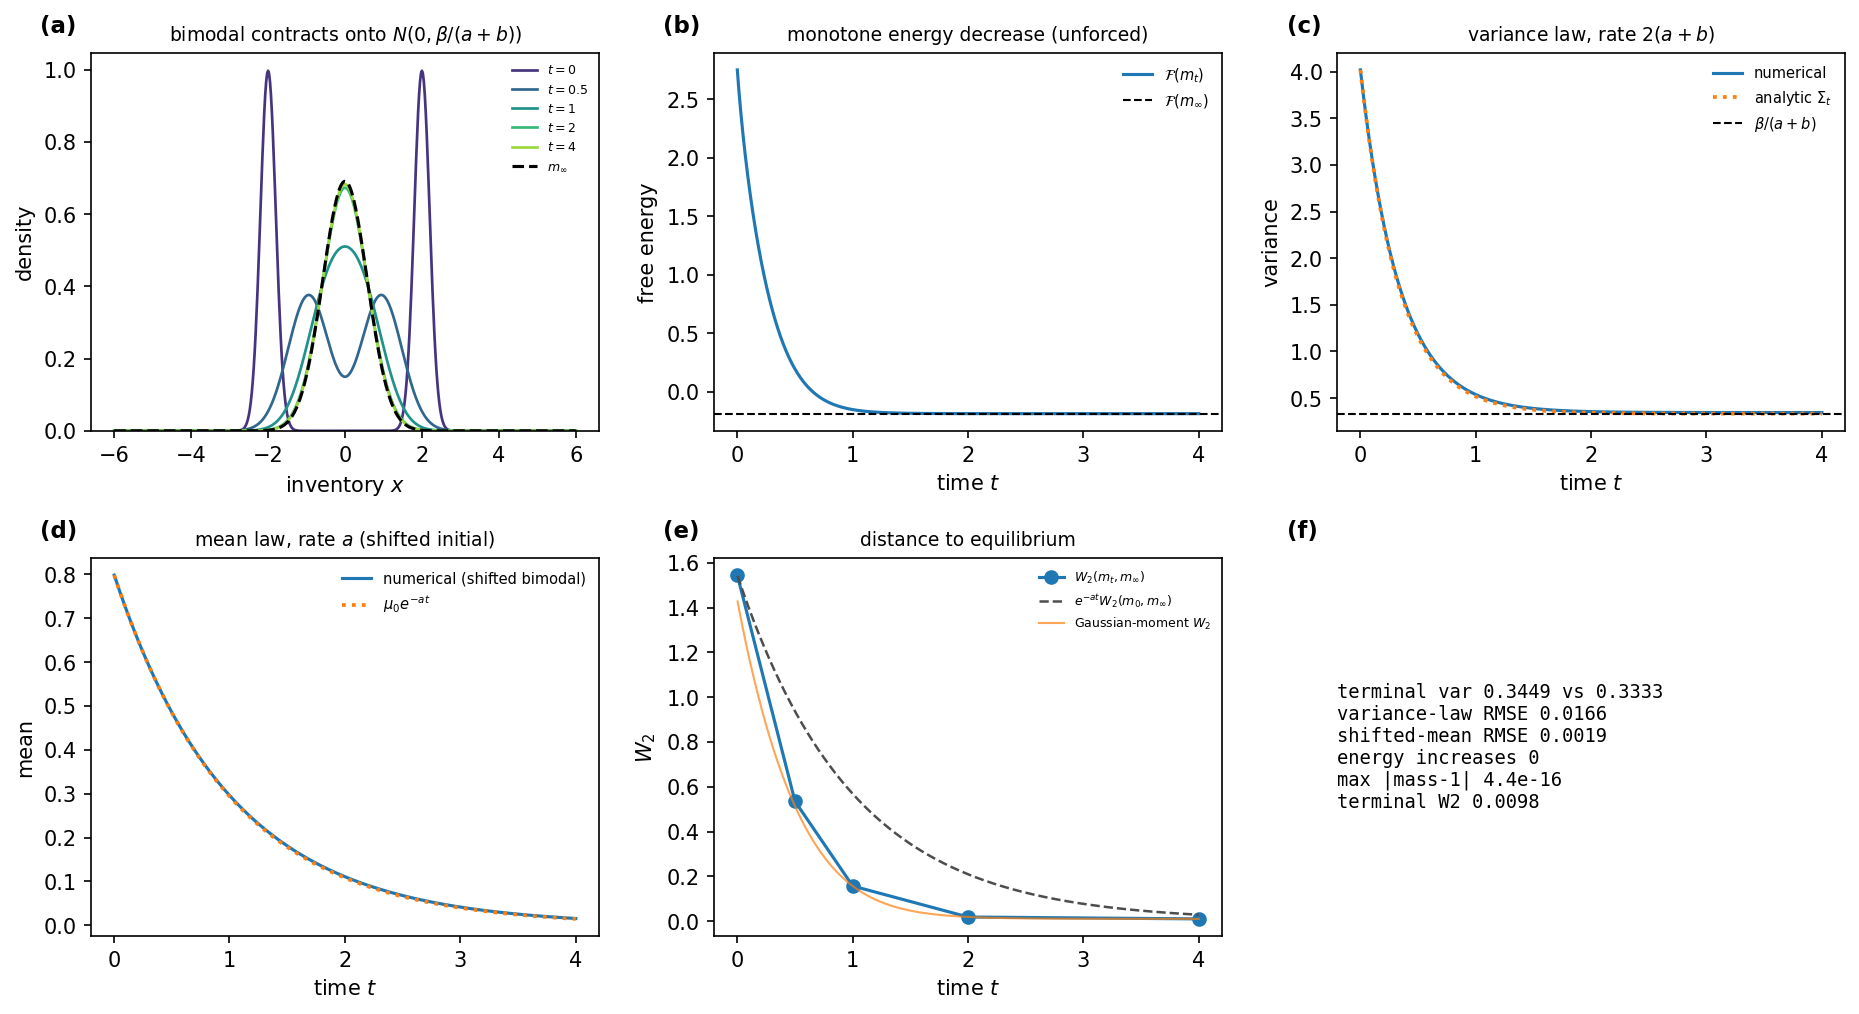
\includegraphics[width=\linewidth]{exp01_relaxation.png}
\caption{Non-Gaussian relaxation of a bimodal inventory law onto $N(0,1/3)$.
Energy decreases monotonically; variance tracks the closed-form ODE. This is a
numerical check of Theorem~\ref{thm:gauss}, not a market observation.}
\label{fig:exp01}
\end{figure}

The paper bimodal is mean-zero, so $\mu_t=\mu_0 e^{-at}$ is nearly vacuous there.
A shifted bimodal companion,
$\tfrac12 N(-1.2,0.2^2)+\tfrac12 N(2.8,0.2^2)$, yields a mean-law RMSE of
$0.0019$ against $\mu_0 e^{-at}$.

\subsection{Liquidity shock}
\label{sec:exp-shock}

Starting from equilibrium, we apply a transient tilt
$V_t(x)=\frac{a}{2}(x-c_t)^2$ with $c_t=2$ on $t\in[2,4]$ and $c_t=0$
otherwise. The mean reaches $1.720$ at the end of the window, against the
quasi-static prediction $c(1-e^{-a\Delta T})=2(1-e^{-2})\approx 1.729$, and then
decays toward zero at rate $a$ (Figure~\ref{fig:exp02}).

Because $V_t$ is time-dependent, the unadjusted functional $F$ is not a Lyapunov
function on the forcing window. The system can follow the correct instantaneous
Wasserstein gradient while $F(m_t)$ rises: external forcing injects energy. In
this run $F$ increased on all $1000$ forced steps and had zero energy-increasing
steps after the tilt was removed. Autonomous dissipation
(Theorem~\ref{thm:jko}) and externally forced dynamics must be distinguished.

\begin{figure}[t]
\centering

\includegraphics[width=\linewidth]{exp02_shock.png}
\caption{Liquidity shock via a time-dependent tilt of $V$. The mean tracks the
quasi-static prediction; unadjusted $F$ rises on every forced step and decreases
once the tilt is removed.}
\label{fig:exp02}
\end{figure}

\subsection{Interaction-strength sweep}
\label{sec:exp-sweep}

We vary the interaction $b$ over $[0,3]$ and also sweep $a$ and $\beta$,
starting from $N(1,1)$ so that the mean law is identifiable. Numerical
equilibrium variance decreases in $b$ and tracks $\beta/(a+b)$, with a maximum
absolute error of $0.021$ on the $b$-sweep (a coarser grid than
Section~\ref{sec:exp-relax}). Fitted mean rates recover $a$ with MAE $0.029$
(Figure~\ref{fig:exp03}). We emphasize the comparative static: larger $b$ is a
cross-sectional \emph{dispersion penalty} that compresses inventories, not a
penalty on dealers holding similar positions.

\begin{figure}[t]
\centering
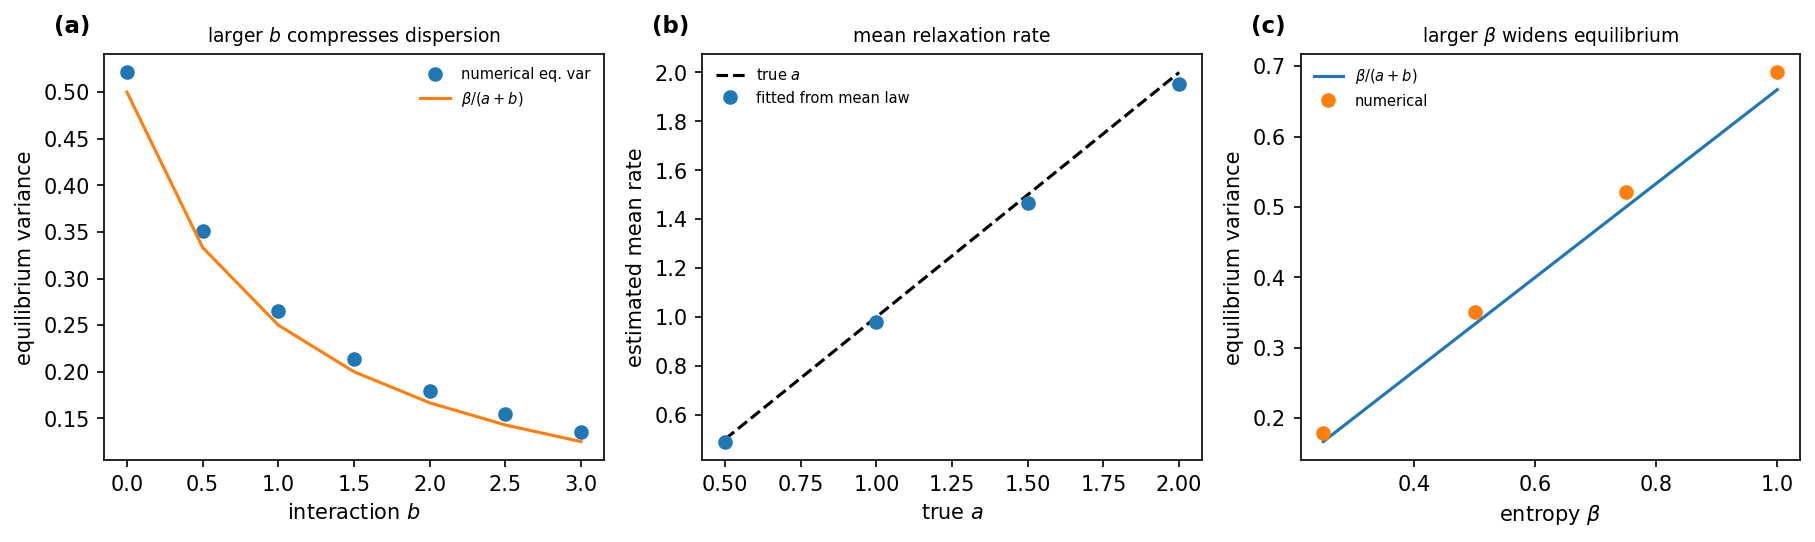
\includegraphics[width=\linewidth]{exp03_parameter_sweep.png}
\caption{Comparative statics in the interaction strength $b$: equilibrium
variance decreases as $b$ increases and tracks $\beta/(a+b)$.}
\label{fig:exp03}
\end{figure}

\subsection{Solver comparison}
\label{sec:exp-solvers}

We compare explicit FP, implicit FP, and quantile JKO over a small grid of
spatial resolutions, time steps, and JKO quantile sizes, reporting runtime,
moment error relative to Theorem~\ref{thm:gauss}, $\Wtwo$ to $m_\infty$, mass
error, positivity, and energy-increasing steps (Figure~\ref{fig:exp04}). The
useful question is not whether explicit Euler fails above CFL---that is
expected---but whether respecting the Wasserstein structure gives the guarantees
of Theorem~\ref{thm:jko} relative to a stable Eulerian alternative.

Explicit FP at $1.8\times$ the diffusive CFL limit develops negative mass and
diverges. Implicit FP remains stable, conserves mass to $\sim 10^{-15}$, and
dissipates $F$, with numerical diffusion visible in the variance law. JKO
preserves mass and positivity exactly, dissipates $F$ at every step, and has no
CFL restriction. We \emph{do not} claim that JKO is more accurate at equal
spatial resolution: the quantile mesh, proximal step $\tau$, and Eulerian
$\Delta t$ are different discretizations. A fair accuracy ranking would require a
matched compute/error study, which we have not run.
Table~\ref{tab:solvers} records the structural comparison only.

\begin{table}[t]
\centering
\caption{Discretizations of the autonomous quadratic flow. ``CFL'' is the
explicit diffusive restriction $\Delta t\le (\Delta x)^2/(2\beta)$. We do not
interpret terminal $\Wtwo$ at unmatched resolution as an accuracy ranking.}
\label{tab:solvers}
\begin{tabular}{lccc}
\hline
 & Explicit FP & Implicit FP & Quantile JKO \\
\hline
Stable above CFL & no & yes & yes (no CFL) \\
Mass conserved & no & to $\sim 10^{-15}$ & exact \\
Positivity & fails & stable, numerical diffusion & exact \\
Energy-increasing steps & diverges & $0$ & $0$ \\
\hline
\end{tabular}
\end{table}

\begin{figure}[t]
\centering

\includegraphics[width=\linewidth]{exp04_solver_benchmark.png}
\caption{JKO versus explicit and implicit Fokker--Planck integrators. JKO
preserves mass and positivity and dissipates $F$ with no CFL restriction. We do
not rank accuracy at unmatched resolution.}
\label{fig:exp04}
\end{figure}

\section{Synthetic diagnostics and a template for empirical tests}
\label{sec:diagnostics}

Dealer inventories are not observed at the population level, so this section is
not an empirical study of markets. It records a suite of synthetic tests that
\emph{would} be run, in this order, on an observable market-state distribution,
and it checks that the tests accept data generated by $F$ and reject several
deliberately wrong dynamics.

A general mean-field market-making game need not be a Wasserstein gradient flow
(Remark~\ref{rem:scope}). Even under~\eqref{eq:mv}, cosine alignment cannot carry
the empirical claim by itself. We treat three complementary diagnostics.

\paragraph{Moment restrictions (first).}
The quadratic model gives low-dimensional, hard-to-hide predictions. On a
training segment only, estimate $a$ from consecutive means and $(a+b)$,
$\sigma_\infty^2$ from consecutive variances; then test out of sample
\begin{align}
  \mu_{t+\Delta t}
  &\stackrel{?}{\approx}
  e^{-a\Delta t}\mu_t,
  \label{eq:mean-restrict}\\
  \Sigma_{t+\Delta t}
  &\stackrel{?}{\approx}
  \frac{\beta}{a+b}
  +
  e^{-2(a+b)\Delta t}
  \Bigl(\Sigma_t-\frac{\beta}{a+b}\Bigr).
  \label{eq:var-restrict}
\end{align}
If~\eqref{eq:mean-restrict}--\eqref{eq:var-restrict} fail badly out of sample,
that is the result; a more flexible score estimator should not be used to hide
it.

On McKean--Vlasov particles generated from the true $(a,b,\beta)$, a
chronological split recovers $\hat a=0.984$ (true $1$) and
$\widehat{a+b}=1.455$ (true $1.5$), with out-of-sample mean MAE $0.004$ and
variance MAE $0.008$ (Figure~\ref{fig:exp06}).

\begin{figure}[t]
\centering
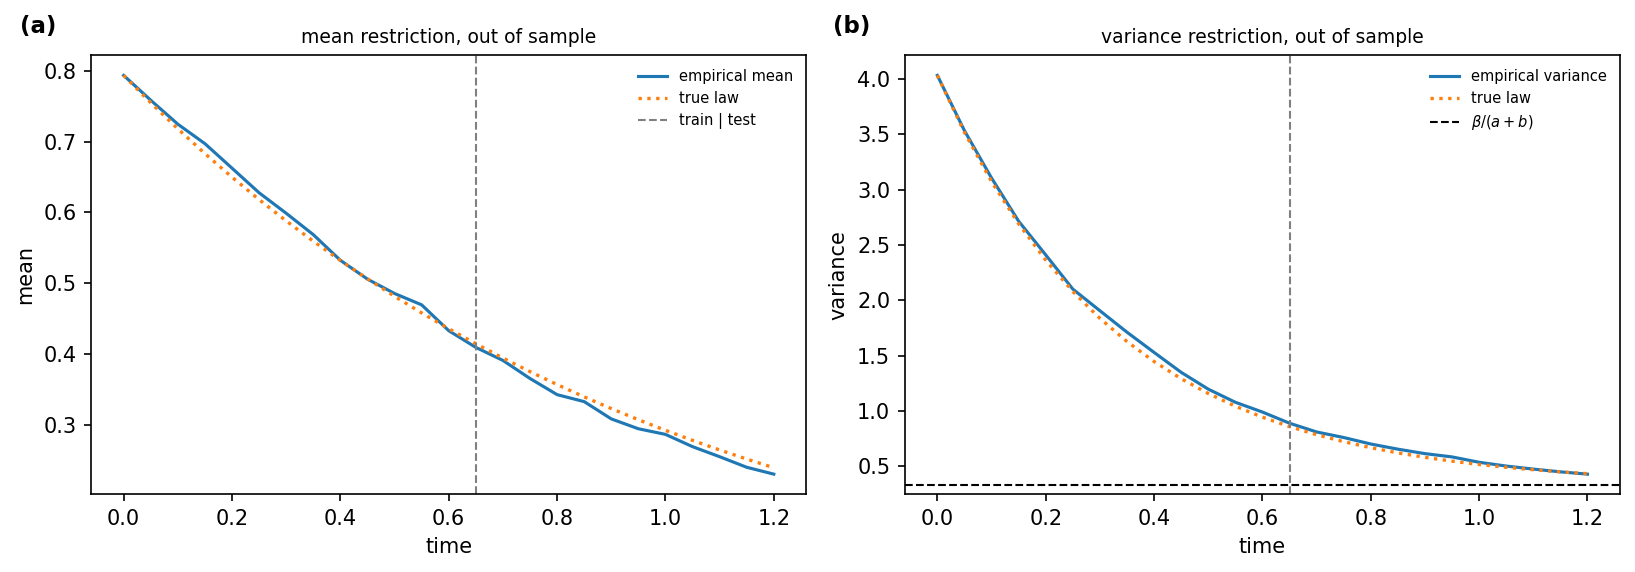
\includegraphics[width=\linewidth]{exp06_moment_validation.png}
\caption{Train-then-test moment restrictions on synthetic McKean--Vlasov
particles. Out-of-sample mean and variance increments match the closed-form
laws. Not a test on market inventories.}
\label{fig:exp06}
\end{figure}

\paragraph{Distribution forecasting (second).}
Given $D_t$, form $\widehat D_{t+\Delta t}$ from the fitted flow (Gaussian
moment matching, or one JKO step) and compare
$\Wtwo(\widehat D_{t+\Delta t},D_{t+\Delta t})$ to persistence and to a
no-interaction ($b=0$) baseline. Parameters are estimated only on past windows.

On the same synthetic flow, mean one-step $\Wtwo$ is $0.064$ for persistence,
$0.045$ for affine moment matching, $0.048$ for $b=0$, and $0.036$ for one JKO
step (Figure~\ref{fig:exp07}). When the data really are generated by the model,
the model contains predictive information beyond carrying the previous cloud
forward. (A short, far-from-equilibrium training window can still mis-identify
$\sigma_\infty^2$; local increments may forecast even when the Gibbs variance is
not recovered.)

\begin{figure}[t]
\centering
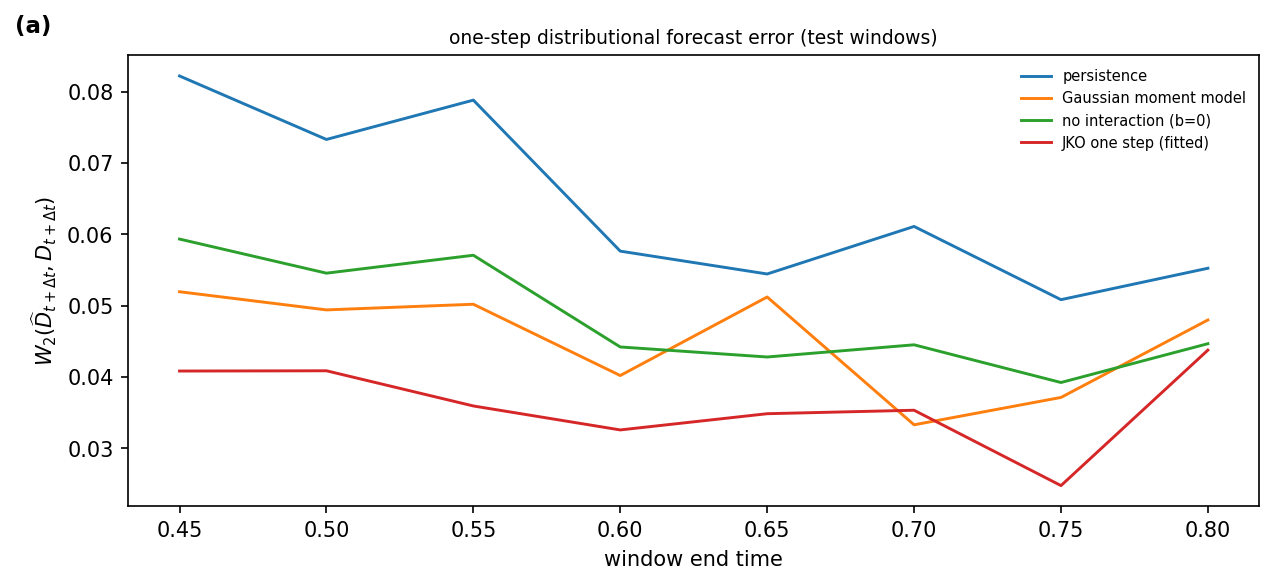
\includegraphics[width=\linewidth]{exp07_distribution_forecast.png}
\caption{One-step $\Wtwo$ forecasts on synthetic data generated by the model.
JKO ($0.036$) and moment matching beat persistence ($0.064$). A synthetic sanity
check, not an empirical finding.}
\label{fig:exp07}
\end{figure}

\paragraph{Local directional alignment (third).}
For consecutive empirical clouds $(D_t,D_{t+\Delta t})$, let $T$ be the
one-dimensional monotone (Brenier) map and $u_{\mathrm{obs}}=T-\mathrm{id}$ the
displacement of the two \emph{marginals}. This is not the trajectory of labeled
dealers unless identities are observed. The predicted Otto velocity is
\[
  v_{\mathrm{pred}}(x)
  =
  -(a+b)x+b\mu_t-\beta\nabla\log\rho_t(x).
\]
In $L^2(D_t)$ we report the signed cosine
\[
  \cos\theta
  =
  \frac{\langle u_{\mathrm{obs}},v_{\mathrm{pred}}\rangle}
  {|u_{\mathrm{obs}}|\,|v_{\mathrm{pred}}|},
\]
the best-fit scale
$\hat\lambda=\langle u_{\mathrm{obs}},v_{\mathrm{pred}}\rangle/|v_{\mathrm{pred}}|^2$,
and the unexplained Wasserstein displacement
$|u_{\mathrm{obs}}-\hat\lambda v_{\mathrm{pred}}|^2/|u_{\mathrm{obs}}|^2=1-\cos^2\theta$.
We do not call the residual rotational: in one dimension, and from marginals
alone, microscopic circulation is not identifiable.

Alignment is an interpretability diagnostic for whatever predictive success the
first two tests obtain, not a substitute for them. Two synthetic facts make this
precise.

\emph{Window size is testable.} The gradient $v_{\mathrm{pred}}$ is an
instantaneous tangent; OT between $D_t$ and $D_{t+\Delta t}$ is a finite
displacement. On the true flow, mean $\cos\theta$ is $0.87$ at $\Delta t=0.05$
and $0.35$ at $\Delta t=0.40$ (Figure~\ref{fig:exp08}), with later large windows
changing sign. Directional agreement is a local statement; $\Delta t$ is not a
pure nuisance that cosine removes.

\emph{Cosine is blind to overall scale.} The map
$(a,b,\beta)\mapsto c(a,b,\beta)$ multiplies $v_{\mathrm{pred}}$ by $c$ and
leaves $\cos\theta$ unchanged. Evaluating the true trajectory at deliberately
wrong parameters moves cosine only from $0.88$ to $0.81$, while variance MAE
jumps from $0.019$ to $0.38$ (Figure~\ref{fig:exp05}). Moment restrictions
recover the missing timescale; alignment does not. That is a reason to
run~\eqref{eq:mean-restrict}--\eqref{eq:var-restrict} first, not an
implementation footnote.

On deliberately wrong generators (nonlinear $\tanh$ drift, omitted constant
force, anti-gradient, rigid translation) cosine and/or the moment laws
deteriorate, as they should. State-dependent diffusion with the correct drift
still yields cosine $\approx 0.69$: the score term is not a sharp test of
$\beta$.

\begin{figure}[t]
\centering

\includegraphics[width=0.85\linewidth]{exp05_synthetic_falsification.png}
\caption{Synthetic falsification: cosine and moment errors on the true flow
versus misspecified generators. Wrong overall scale barely moves cosine while
wrecking the variance law.}
\label{fig:exp05}
\end{figure}

\begin{figure}[t]
\centering

\includegraphics[width=\linewidth]{exp08_directional_alignment.png}
\caption{Directional alignment versus window size $\Delta t$ on the true flow.
Cosine falls from $\approx 0.87$ at $0.05$ to $\approx 0.35$ at $0.40$: the
gradient is a local tangent, OT a finite displacement.}
\label{fig:exp08}
\end{figure}

If an observable market-state distribution becomes available, we would run the
three diagnostics in the order above, with chronological train/test splits and
control distributions for cosine. Until then, Claim~3---empirical relevance for
markets---remains open.

\section{Conclusion}
\label{sec:conclusion}

In a one-dimensional quadratic mean-field inventory model, the population density
is the $2$-Wasserstein gradient flow of an explicit free energy
(Proposition~\ref{prop:gf}); JKO inherits mass conservation, positivity, and
monotone energy dissipation unconditionally in the step size on the
\emph{autonomous} problem (Theorem~\ref{thm:jko}); equilibria are
McKean--Vlasov--Gibbs densities (Proposition~\ref{prop:eq}); and
$N(0,\beta/(a+b))$ together with rates $a$ and $2(a+b)$ are available in closed
form (Theorem~\ref{thm:gauss}). Numerical experiments confirm these predictions.
JKO preserves probability structure and dissipates $F$ without a CFL
restriction. Explicit finite differences fail above CFL, as expected. We do not
claim accuracy superiority at equal resolution.

The interaction $W=\frac{b}{2}(x-y)^2$ with $b>0$ penalizes cross-sectional
dispersion. A time-dependent tilt can raise the unadjusted energy while the state
still follows the instantaneous gradient; Lyapunov decrease is an autonomous
property.

What remains open is whether any observed market-state distribution is usefully
approximated by descent of this $F$. The diagnostics
above---moment restrictions, distributional forecasting, and local directional
alignment---are a template for that test, not a substitute for it. A general
market-making mean-field game is not a Wasserstein gradient flow. The quadratic
specification is the one that makes the structure exact; richer costs need not be
potential.

\paragraph{Limitations.}
Dealer inventories are not directly observable at the population level; the
quadratic specification is the one that makes the gradient-flow structure exact;
and, as stressed in Remark~\ref{rem:scope}, a general market-making MFG is
\emph{not} a Wasserstein gradient flow. The closed-form Gaussian results rely on
the quadratic interaction, and the 1D quantile solver does not extend directly to
high-dimensional agent states.

\bibliographystyle{plainnat}
\begin{thebibliography}{99}

\bibitem[Ambrosio, Gigli, and Savar\'e(2008)]{AGS08}
L.~Ambrosio, N.~Gigli, and G.~Savar\'e.
\newblock \emph{Gradient Flows in Metric Spaces and in the Space of Probability
Measures}.
\newblock Birkh\"auser, 2nd edition, 2008.

\bibitem[Avellaneda and Stoikov(2008)]{AvellanedaStoikov08}
M.~Avellaneda and S.~Stoikov.
\newblock High-frequency trading in a limit order book.
\newblock \emph{Quantitative Finance}, 8(3):217--224, 2008.

\bibitem[Benamou and Brenier(2000)]{BenamouBrenier00}
J.-D. Benamou and Y.~Brenier.
\newblock A computational fluid mechanics solution to the Monge--Kantorovich
mass transfer problem.
\newblock \emph{Numerische Mathematik}, 84:375--393, 2000.

\bibitem[Brenier(1991)]{Brenier91}
Y.~Brenier.
\newblock Polar factorization and monotone rearrangement of vector-valued
functions.
\newblock \emph{Communications on Pure and Applied Mathematics}, 44(4):375--417,
1991.

\bibitem[Cardaliaguet]{CardaliaguetNotes}
P.~Cardaliaguet.
\newblock Notes on mean field games.
\newblock Technical report, 2013.

\bibitem[Gu\'eant, Lehalle, and Fernandez-Tapia(2013)]{GueantLehalleFernandez2013}
O.~Gu\'eant, C.-A. Lehalle, and J.~Fernandez-Tapia.
\newblock Dealing with the inventory risk: a solution to the market making
problem.
\newblock \emph{Mathematics and Financial Economics}, 7:477--507, 2013.

\bibitem[Horv\'ath, Kokoszka, and Rice(2014)]{HorvathKokoszka}
L.~Horv\'ath, P.~Kokoszka, and G.~Rice.
\newblock Testing stationarity of functional time series.
\newblock \emph{Journal of Econometrics}, 179(1):66--82, 2014.

\bibitem[Jordan, Kinderlehrer, and Otto(1998)]{JKO98}
R.~Jordan, D.~Kinderlehrer, and F.~Otto.
\newblock The variational formulation of the Fokker--Planck equation.
\newblock \emph{SIAM Journal on Mathematical Analysis}, 29(1):1--17, 1998.

\bibitem[Mokrov et al.(2021)]{JKOflow}
P.~Mokrov, A.~Korotin, L.~Li, A.~Kolesnikov, and E.~Burnaev.
\newblock Large-scale Wasserstein gradient flows.
\newblock In \emph{Advances in Neural Information Processing Systems}, 2021.

\bibitem[Lasry and Lions(2007)]{LasryLions07}
J.-M. Lasry and P.-L. Lions.
\newblock Mean field games.
\newblock \emph{Japanese Journal of Mathematics}, 2:229--260, 2007.

\bibitem[McCann(1997)]{McCann97}
R.~J. McCann.
\newblock A convexity principle for interacting gases.
\newblock \emph{Advances in Mathematics}, 128(1):153--179, 1997.

\bibitem[Otto(2001)]{Otto01}
F.~Otto.
\newblock The geometry of dissipative evolution equations: the porous medium
equation.
\newblock \emph{Communications in Partial Differential Equations},
26(1--2):101--174, 2001.

\bibitem[Peyr\'e and Cuturi(2019)]{PeyreCuturi19}
G.~Peyr\'e and M.~Cuturi.
\newblock Computational optimal transport.
\newblock \emph{Foundations and Trends in Machine Learning}, 11(5--6):355--607,
2019.

\bibitem[Santambrogio(2015)]{Santambrogio15}
F.~Santambrogio.
\newblock \emph{Optimal Transport for Applied Mathematicians}.
\newblock Birkh\"auser, 2015.

\bibitem[Villani(2003)]{Villani03}
C.~Villani.
\newblock \emph{Topics in Optimal Transportation}.
\newblock AMS, 2003.

\end{thebibliography}

\appendix

\section{Proofs}
\label{app:proofs}

We collect the proofs of the results of Section~\ref{sec:results}. Throughout,
$F$ is the quadratic free energy~\eqref{eq:Fquad} on $\Ptwo(\R)$, and we write
$\mu(\rho)=\int x\,\rho\,dx$ and
$\Sigma(\rho)=\int x^2\rho\,dx-\mu(\rho)^2$ for the mean and variance.

\subsection{Proof of Proposition~\ref{prop:gf}}

We first compute the first variation of~\eqref{eq:Fquad}. For the interaction
term, perturbing $\rho\mapsto\rho+\varepsilon\chi$ with $\int\chi=0$ and
collecting the $O(\varepsilon)$ term, the symmetric kernel contributes
$\int(W\ast\rho)\,\chi$, so the interaction first variation is $W\ast\rho$.
Together with the elementary variations of the potential and entropy terms,
\begin{equation}
\label{eq:dF-app}
\frac{\delta F}{\delta\rho}(x)
=
V(x)+(W\ast\rho)(x)+\beta\bigl(\log\rho(x)+1\bigr),
\end{equation}
in agreement with~\eqref{eq:dF}. For the quadratic data~\eqref{eq:quad},
\[
(W\ast\rho)(x)
=
\int\frac{b}{2}(x-y)^2\rho(y)\,dy
=
\frac{b}{2}\Bigl(x^2-2x\mu(\rho)+\int y^2\rho\,dy\Bigr),
\]
whence $\nabla(W\ast\rho)(x)=b(x-\mu(\rho))$ and $\nabla V(x)=ax$. Therefore
\[
\nabla\frac{\delta F}{\delta\rho}(x)
=
(a+b)x-b\mu(\rho)+\beta\frac{\nabla\rho}{\rho}.
\]
Substituting into~\eqref{eq:gf} yields~\eqref{eq:mv}. Writing this as
$\partial_t m_t=-\partial_x(v_t m_t)+\beta\partial_{xx}m_t$ identifies
$v_t(x)=-(a+b)x+b\mu_t$.

For the mean-field-game statement, recall that in a potential game the coupling
is a first variation, $f(x,m)=\delta G/\delta m$, and the forward equation
of~\eqref{eq:mfg} is the continuity equation with drift $-D_p H(x,\nabla u)$. If
the running cost and the Hamiltonian are chosen so that the equilibrium feedback
reproduces the drift $-\nabla(V+W\ast m)$---as is the case for a quadratic
inventory cost with the mean-field penalty
$\frac12\iint W\,mm$---then the forward equation is
precisely~\eqref{eq:mv}.\qed

\subsection{Proof of Theorem~\ref{thm:jko}}

(i) \emph{Existence and uniqueness.}
The map $\rho\mapsto\frac1{2\tau}\Wtwo^2(\rho,\rho_k)$ is lower semicontinuous
for the narrow topology and has $W_2$-bounded sublevel sets; $F$ is lower
semicontinuous and bounded below on $\Ptwo(\R)$ (the entropy is controlled by the
second moment via the Gaussian, and $V,W\ge 0$). Hence the JKO objective is
l.s.c.\ with compact sublevel sets and a minimizer exists by the direct
method~\cite{AGS08}. For uniqueness, by Theorem~\ref{thm:gauss}(iii) the
functional $F$ is $a$-geodesically convex with $a>0$, and
$\rho\mapsto\frac1{2\tau}\Wtwo^2(\rho,\rho_k)$ is $\frac1\tau$-geodesically
convex along generalized geodesics; the sum is strictly convex, so the minimizer
is unique~\cite[Ch.~4]{AGS08}.

\emph{Absolute continuity and positivity.}
If $\rho_{k+1}$ had a singular part, replacing it by its absolutely continuous
regularization strictly decreases the entropy while changing $\Wtwo^2(\cdot,\rho_k)$
and the other terms by an arbitrarily small amount, contradicting minimality;
hence $\rho_{k+1}\ll\mathrm{Leb}$. The optimality condition for~\eqref{eq:jko-step}
reads, with $\phi_k$ the Kantorovich potential from $\rho_{k+1}$ to $\rho_k$,
\[
\frac{\delta F}{\delta\rho}(\rho_{k+1})(x)+\frac{\phi_k(x)}{\tau}
=\mathrm{const}
\quad\text{on }\mathrm{supp}(\rho_{k+1}).
\]
Inserting~\eqref{eq:dF-app} and solving for the density yields a strictly
positive Gibbs form.

(ii) \emph{Mass and positivity.}
The minimization is over $\Ptwo(\R)$, so $\rho_{k+1}$ is by definition a
probability measure. No discretization of the flux is involved, so these hold
exactly.

(iii) \emph{Energy dissipation.}
Since $\rho_{k+1}$ minimizes the objective and $\rho_k$ is admissible with
$\Wtwo(\rho_k,\rho_k)=0$,
\[
F(\rho_{k+1})+\frac{1}{2\tau}\Wtwo^2(\rho_{k+1},\rho_k)
\le
F(\rho_k),
\]
which is~\eqref{eq:edp}; in particular $F(\rho_{k+1})\le F(\rho_k)$.

(iv) \emph{Convergence as $\tau\to 0$.}
Estimate~\eqref{eq:edp} is the discrete energy-dissipation inequality of the
minimizing-movements scheme. Summing it yields the total-square-distance bound
$\sum_k \Wtwo^2(\rho_{k+1},\rho_k)\le 2\tau(F(\rho_0)-\inf F)$, which gives
equicontinuity of the piecewise-constant interpolants; by the refined Ascoli
theorem in $(\Ptwo,W_2)$ a subsequence converges uniformly to an absolutely
continuous curve, and the $a$-convexity of $F$ identifies the limit as the unique
gradient flow of~\eqref{eq:mv}~\cite[Thm.~11.1.6 and Thm.~4.0.4]{AGS08};
uniqueness of the limit promotes convergence of the whole family.\qed

\subsection{Proof of Proposition~\ref{prop:eq}}

A measure $m_\infty$ is stationary for~\eqref{eq:gf} iff
$\nabla\cdot\bigl(m_\infty\nabla\delta F/\delta\rho(m_\infty)\bigr)=0$. Testing
against $\delta F/\delta\rho(m_\infty)$ and integrating by parts forces
$\nabla\delta F/\delta\rho(m_\infty)=0$ $m_\infty$-a.e., i.e.\
$\delta F/\delta\rho(m_\infty)$ is constant on $\mathrm{supp}(m_\infty)$.
Conversely a constant first variation makes the drift vanish. Setting
\eqref{eq:dF-app} equal to a constant and solving yields~\eqref{eq:gibbs}.\qed

\subsection{Proof of Theorem~\ref{thm:gauss}}

(i) \emph{Equilibrium.}
For the quadratic data, $(W\ast m_\infty)(x)=\frac{b}{2}(x^2-2x\mu_\infty+\int y^2 m_\infty)$
with $\mu_\infty=\mu(m_\infty)$. The effective potential in~\eqref{eq:gibbs} is
therefore quadratic in $x$,
\[
V(x)+(W\ast m_\infty)(x)
=
\frac{a+b}{2}x^2-b\mu_\infty x+\mathrm{const},
\]
so $m_\infty$ is Gaussian. Completing the square, its mean is
$b\mu_\infty/(a+b)$; self-consistency forces $\mu_\infty=0$ since $a>0$. The
coefficient of $x^2$ is $(a+b)/(2\beta)$, giving variance
$\sigma_\infty^2=\beta/(a+b)$. Uniqueness follows from
Proposition~\ref{prop:eq} together with strict convexity.

(ii) \emph{Moment dynamics.}
Multiply~\eqref{eq:mv} in the form $\partial_t m=-\partial_x(vm)+\beta\partial_{xx}m$,
$v(x)=-(a+b)x+b\mu_t$, by $x$ and integrate:
$\dot\mu_t=\int v\,m_t\,dx=-(a+b)\mu_t+b\mu_t=-a\mu_t$,
so $\mu_t=\mu_0 e^{-at}$. Multiplying instead by $x^2$ and writing
$S_t=\int x^2 m_t$,
$\dot S_t=-2(a+b)S_t+2b\mu_t^2+2\beta$.
With $\Sigma_t=S_t-\mu_t^2$ and $\frac{d}{dt}(\mu_t^2)=-2a\mu_t^2$,
\[
\dot\Sigma_t
=
\dot S_t-2\mu_t\dot\mu_t
=
-2(a+b)\Sigma_t+2\beta,
\]
where the $\mu_t^2$ terms cancel because $-2(a+b)+2b+2a=0$. Integrating gives
the variance law in~\eqref{eq:moments}.

(iii) \emph{Displacement convexity and contraction.}
By McCann's criterion~\cite{McCann97}, on $(\Ptwo(\R),\Wtwo)$ the internal
energy $\beta\int\rho\log\rho$ is geodesically convex; the potential energy
$\int V\rho$ is $a$-geodesically convex since $V''=a$; and the interaction
energy with $W(z)=\frac{b}{2}z^2$ convex is geodesically convex. Summing, $F$ is
$a$-geodesically convex. The general theory of gradient flows of $\lambda$-convex
functionals then yields the exponential contraction~\cite[Thm.~11.2.1]{AGS08},
and the corresponding contraction of the resolvent (JKO) operator. The rate is
sharp: by~\eqref{eq:moments} the mean is the slowest mode, relaxing at exactly
$a$ while the variance relaxes faster at $2(a+b)$.\qed

\section{On the one-dimensional JKO discretization}
\label{app:jko1d}

In one dimension the optimal transport between $\rho$ and $\rho_k$ is the
monotone rearrangement, and
$\Wtwo^2(\rho,\rho_k)=\int_0^1\bigl(Q_\rho(u)-Q_{\rho_k}(u)\bigr)^2\,du$
where $Q_\rho=F_\rho^{-1}$ is the quantile function. Pushing the free energy
through this change of variable, using $\rho(Q(u))=1/Q'(u)$, gives
\[
F[Q]
=
\frac{a}{2}\int_0^1 Q(u)^2\,du
+
\frac{b}{2}\Bigl(\int_0^1 Q^2-\Bigl(\int_0^1 Q\Bigr)^2\Bigr)
-
\beta\int_0^1\log Q'(u)\,du,
\]
so that each JKO step is the strictly convex program
$\min_Q\, F[Q]+\frac1{2\tau}\int_0^1(Q-Q_k)^2\,du$ over nondecreasing $Q$. We
parametrize monotonicity through nonnegative increments and solve with L-BFGS.
Mass is conserved and positivity ($Q'>0$) is enforced exactly by construction,
which is why the JKO column of Table~\ref{tab:solvers} attains exact mass
conservation and positivity. In higher dimensions the monotone rearrangement is
unavailable and one resorts to entropic regularization of the proximal
step~\cite{PeyreCuturi19}.

\end{document}
